\documentclass{beamer}
\usepackage{amsmath}
\usepackage{mathtools}
\usepackage{amsfonts}
\usepackage{amssymb}
\usepackage{graphicx}

% Lightweight replacements for the gvv package commands used in this document
\newcommand{\myvec}[1]{\begin{pmatrix}#1\end{pmatrix}}
\newcommand{\rank}{\operatorname{rank}}
\renewcommand{\vec}[1]{\mathbf{#1}}

\title{Question 4.2.3}
\author{AI25BTECH11040 - Vivaan Parashar}
\date{\today}

\begin{document}

\frame{\titlepage}

\begin{frame}
    \frametitle{Question: }
    The pair of linear equations:
    \begin{align*}
        2x = 5y + 6 \\
        15y = 6x - 18
    \end{align*}
    represents two lines which are
    \begin{enumerate}
        \item intersecting
        \item parallel
        \item coincident
        \item either intersecting or parallel
    \end{enumerate}
\end{frame}

\begin{frame}
    \frametitle{Solution: }
    To find the type of lines represented by the given pair of linear equations, we first find the solution to the system. If there is a unique solution, the lines are intersecting at one and only one point. If there are infinite solutions, then the lines are coincident. If there are no solutions, then the lines are parallel and not intersecting.

    First the equations can be rewritten in the standard form:
    \begin{align}
        2x - 5y = 6 \tag{1} \\
        6x - 15y = 18 \tag{2}
    \end{align}
    The equations can be written in the form of
    \begin{align}
        \vec{M}\vec{X} = \vec{D} \\
        \implies \myvec{2 & -5   \\ 6 & -15}\myvec{x \\ y} = \myvec{6 \\ 18}
    \end{align}
\end{frame}
\begin{frame}
    To check whether a unique solution exists, we can find the rank of the matrix $\vec{M}$.
    Applying row reduction to $\vec{M}$:
    \begin{align}
        \myvec{2 & -5 \\ 6 & -15} \xleftrightarrow{R_2 \rightarrow R_2 - 3R_1} \myvec{2 & -5 \\ 0 & 0}\\
        \therefore \rank(\vec{M}) = 1
    \end{align}
    Because the rank of $\vec{M}$ is less than the number of rows in the matrix (2), there either exists no solution or an infinite number of solutions. To determine which case it is, we can find the rank of the augmented matrix $\vec{A} = \myvec{\vec{M} & \vec{D}}$.
    Applying row reduction to $\vec{A}$:
    \begin{align}
        \myvec{2 & -5 & 6 \\ 6 & -15 & 18} \xleftrightarrow{R_2 \rightarrow R_2 - 3R_1} \myvec{2 & -5 & 6 \\ 0 & 0 & 0}\\
        \therefore \rank(\vec{A}) = 1
    \end{align}
\end{frame}
\begin{frame}
    Since the rank of the augmented matrix $\vec{A}$ is equal to the rank of the coefficient matrix $\vec{M}$ (1), there exists an infinite number of solutions to the system of equations. Therefore, the lines represented by the given pair of linear equations are coincident.
\end{frame}

\begin{frame}
    \frametitle{Plot: }
    \begin{figure}[h!]
        \centering
        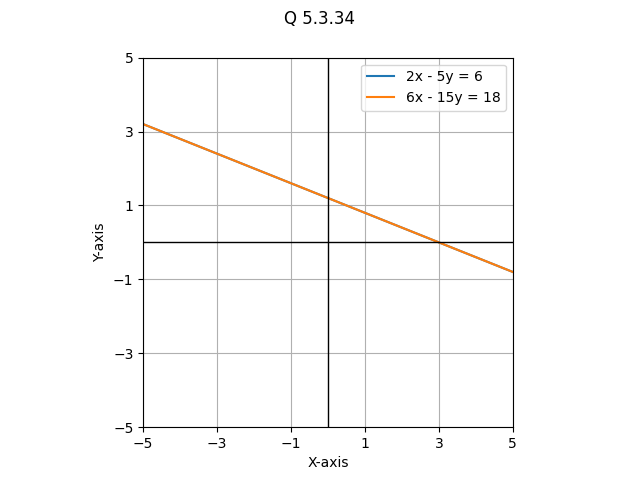
\includegraphics[width=0.9\columnwidth]{../figs/plot.png}
        \caption{Graph of the two coincident lines}
        \label{fig:5.3.34}
    \end{figure}
\end{frame}

\end{document}
